\scanpage{60}
% E: text|upper left first paragraph|Par contre si on fait un tour complet
Par contre, si on fait un tour complet, de façon à revenir à l'orientation de départ de $D$, alors \unsure{évidemment} (c'est le carré du \unsure{lent|petit} demi-tour) on trouve \deleted{\unsure{que alors que ce}} \inserted{un transport parallèle}
% E: diagram|upper left last line of first paragraph|Pol(D) to Pol(D)
\diagram{\begin{tikzcd}\operatorname{Pol}(D)\arrow[r] & \operatorname{Pol}(D)\end{tikzcd}}
% E: text|upper left continuation|qui conserve l'orientation
qui conserve l'orientation.
\deleted{
% E: text|left middle second paragraph|Notons aussi
Notons aussi que \deleted{\unsure{le nb}} pour le ``\unsure{lent|petit} demi-tour autour de $s$'', \deleted{\unsure{comme}} \inserted{quand} le nb de pas est pair, alors le résultat du transport parallèle sur les polygônes des \unsure{positions|portions} donne, sur l'orientation le $=$ résultat que le transport parallèle ordinaire de l'orientation. Cela signifie que l'orientation change \deleted{\unsure{par}} le long de ce \unsure{CCt|Cct}, si $\nu(s)$ pair.
% E: text|left lower paragraph also obliquely cancelled|Si nu(s) impair
Si $\nu(s)$ impair, alors le résultat sur $\operatorname{Pol}(\unsure{D})$, et via transport ordinaire, c'est \deleted{\unsure{pr}} le $=$. \deleted{\unsure{donc}} \inserted{comme} l'orientation est \uline{conservée} par transport parallèle, elle ne l'est pas par transport ordinaire --- donc en tous cas cette dernière change
}
\deleted{
% E: text|right upper continuation|ceci vaut chaque fois
ceci vaut chaque fois qu'on a un circuit fermé sur $X$ (circuit composé de faces) tel que le transport par. ordinaire change l'orientation de \deleted{\unsure{D}} la position \unsure{relative|rectiligne} $D$.
% E: text|right upper middle revised orientation assertion|Alors l'orientation
\deleted{Que le nb d'opérations soit pair \unsure{ne paraît}} \inserted{Alors l'orientation de $X$ change parce que} \unsure{le nb des pas élémentaires est pair}.
% E: text|right middle counting sweeps|Balayer au dessus
Balayer au dessus d'un pt compte comme $2$, balayer au dessus d'une \unsure{p.r.|pce} supersingulière compte comme $1$.
}
% E: text|right lower new assertion|Voilà enfin une façon de voir
Voilà enfin une façon de voir que $\pi_1(\unsure{\widetilde X|\widetilde{\widetilde X}})\longrightarrow\mathbb D_{2n}$ est surjectif.
% E: text|right lower before drawing|On part avec une \unsure{p.r.|por.}
On part avec une \unsure{p.r.|por.} \deleted{\unsure{D D}} \inserted{$D$} proche d'une \unsure{p.r.|por.} supersingulière $D_0$,
% E: drawing|bottom right|green sigmoid D red D0 two red verticals s s prime a
\figure{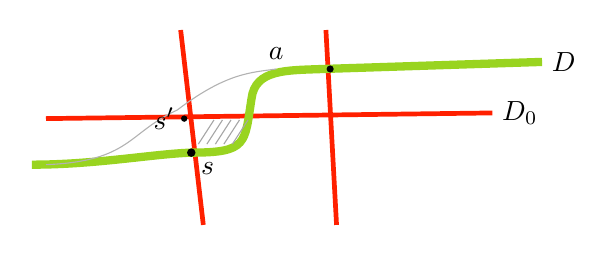
\begin{tikzpicture}[x=.9cm,y=.9cm]
\draw[red!75!orange,line width=1.7pt] (-2.7,0)--(3.6,.08) (-.8,1.25)--(-.48,-1.5) (1.25,1.25)--(1.4,-1.5);
\draw[yellow!60!green,line width=3pt] (-2.9,-.65)..controls (-2,-.65) and (-1.2,-.5)..(-.65,-.48)..controls (.15,-.48) and (.1,-.35)..(.2,.28)..controls (.25,.7) and (.7,.68)..(1.2,.7)--(4.3,.8);
\draw[gray!60] (-2.7,-.65)..controls (-1.5,-.6) and (-1.55,-.2)..(-.85,.12)..controls (-.15,.65) and (.2,.65)..(.55,.7);
\foreach \x in {-.55,-.43,-.31,-.19,-.07}{\draw[gray!70] (\x,-.36)--({\x+.22},-.02);}
\fill (-.65,-.48) circle(.06) (-.75,0) circle(.045) (1.31,.7) circle(.05);
\node[below right] at (-.65,-.48) {$s$};\node[left] at (-.75,0) {$s'$};\node[above] at (.55,.7) {$a$};\node[right] at (4.3,.8) {$D$};\node[right] at (3.6,.08) {$D_0$};
\end{tikzpicture}}
\mspage{59}
